Plots are given in figure \ref{fig:Reg_loc_only}. 
I used the log-likelihood function as my stopping criteria.
For the these non-stochastic experiments I stopped iterating when the improvement in the log-likelihood was less than .001.




\begin{figure}
     \centering
     \begin{subfigure}[b]{0.3\textwidth}
         \centering
         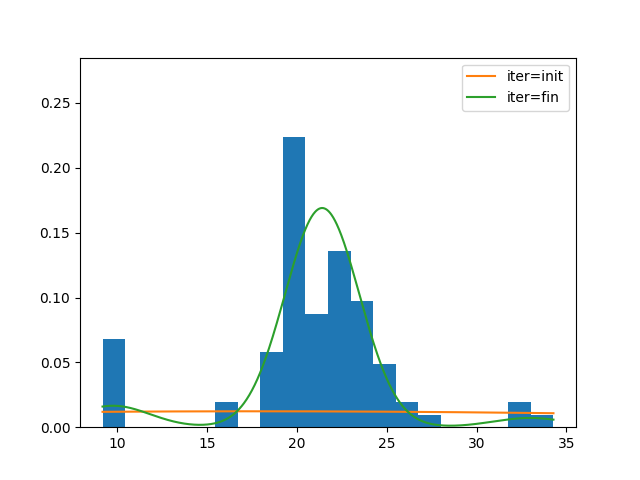
\includegraphics[width=\textwidth]{../code/regular_loc_only_plots/galaxies_hist_k_4.png}
         \caption{K=4}
         \label{fig:Reg_loc_only4}
     \end{subfigure}
     \hfill
     \begin{subfigure}[b]{0.3\textwidth}
         \centering
         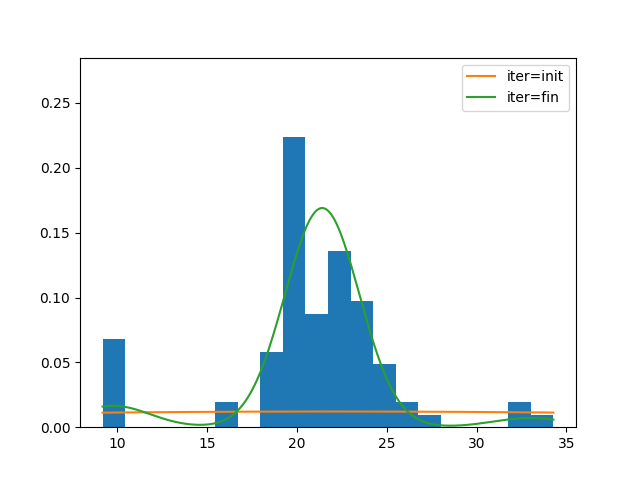
\includegraphics[width=\textwidth]{../code/regular_loc_only_plots/galaxies_hist_k_6.png}
         \caption{K=6}
         \label{fig:Reg_loc_only6}
     \end{subfigure}
     \hfill
     \begin{subfigure}[b]{0.3\textwidth}
         \centering
         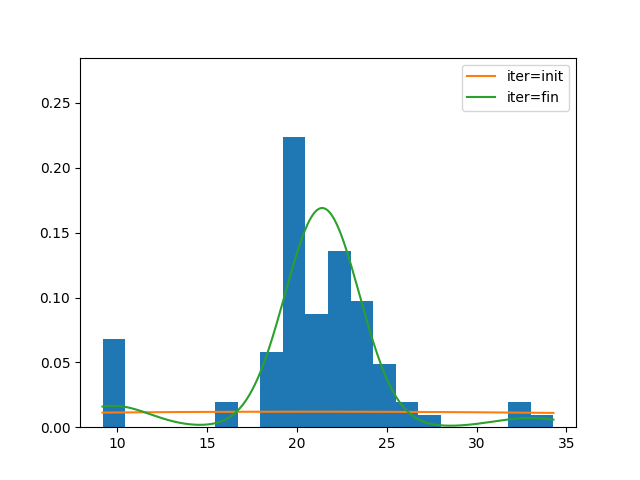
\includegraphics[width=\textwidth]{../code/regular_loc_only_plots/galaxies_hist_k_8.png}
         \caption{K=8}
         \label{fig:Reg_loc_only8}
     \end{subfigure}
     \begin{subfigure}[b]{0.3\textwidth}
         \centering
         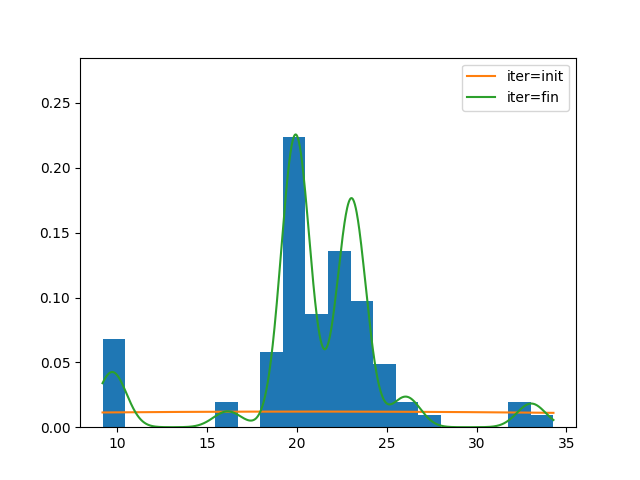
\includegraphics[width=\textwidth]{../code/regular_loc_only_plots/galaxies_hist_k_11.png}
         \caption{K=11}
         \label{fig:Reg_loc_only11}
     \end{subfigure}
     \hfill
     \begin{subfigure}[b]{0.3\textwidth}
         \centering
         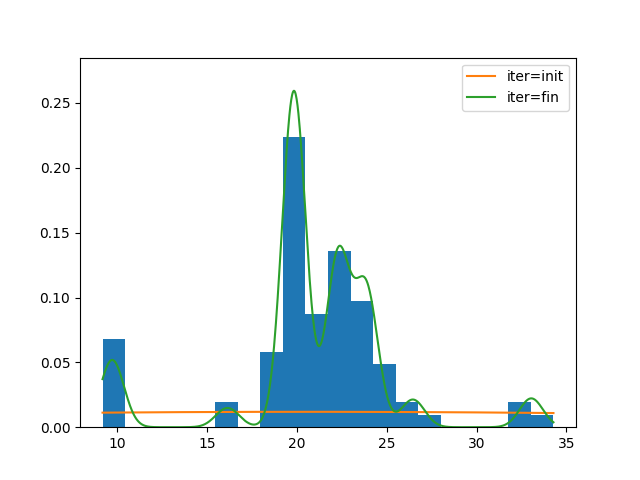
\includegraphics[width=\textwidth]{../code/regular_loc_only_plots/galaxies_hist_k_15.png}
         \caption{K=15}
         \label{fig:Reg_loc_only15}
     \end{subfigure}
     \hfill
     \begin{subfigure}[b]{0.3\textwidth}
         \centering
         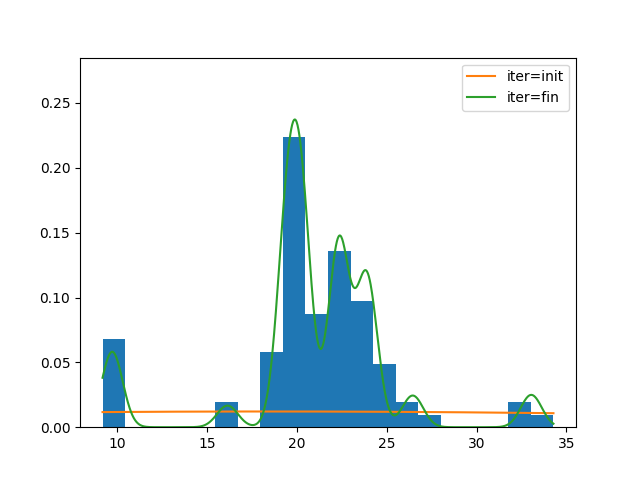
\includegraphics[width=\textwidth]{../code/regular_loc_only_plots/galaxies_hist_k_20.png}
         \caption{K=20}
         \label{fig:Reg_loc_only20}
     \end{subfigure}
        \caption{Non-Stochastic 1-D Location Mixtures}
        \label{fig:Reg_loc_only}
\end{figure}
